\documentclass[conference]{IEEEtran}
% \IEEEoverridecommandlockouts

\usepackage{cite}
\usepackage{amsmath,amssymb,amsfonts}
\usepackage{algorithmic}
\usepackage{graphicx}
\usepackage{textcomp}
\usepackage{xcolor}
\usepackage{tabularx}
\usepackage{array}
\usepackage{subcaption}

\newcolumntype{Y}{>{\raggedright\arraybackslash}X}

\def\BibTeX{{\rm B\kern-.05em{\sc i\kern-.025em b}\kern-.08em
    T\kern-.1667em\lower.7ex\hbox{E}\kern-.125emX}}
\begin{document}

\begin{titlepage}
    \centering

    {\Huge\bfseries Translating clinical narratives into structured evidence\par}
    \vspace{2cm}

    {\large
    A dissertation submitted in partial fulfilment of\par
    The requirement for the degree of\par
    MASTER OF SCIENCE in Artificial Intelligence\par
    in\par
    The Queen’s University of Belfast\par
    by\par
    Conor Brown\par
    4th September 2026
    }
\end{titlepage}


\title{Translating clinical narratives into structured evidence with neuro-symbolic systems\\}



\maketitle

\begin{abstract}
Clinical information extraction (IE) converts clinical 
narratives into structured facts. Large language models can 
do this with significantly less preprocessing than rules-based 
methods, but they introduce new classes of problems: 
hallucination, schema drift and overconfidence. We propose 
a hybrid system where the model extracts entities, interprets 
relations and provides evidence, and the rules normalise 
entities, verify evidence and apply policies to resolve conflicts. 
This modular system preserves the rich uncertainty captured 
in clinical narratives while producing auditable structured 
outputs that confirm to explicit rules. We use 2 public datasets 
of epilepsy letters to evaluate this system on two distinct tasks: 
(1) selecting the most important clinical fact among many and 
(2) building a broad inventory of clinical facts. We show that 
the combined system improved F1 by +0.05 vs. rules-only or 
LLM-only systems, while creating a rich evidence trail with an 
exact evidence score of >0.99. This transparent, 
evidence-grounded system is a step towards making more 
trustworthy systems for clinical use.
\end{abstract}

\begin{IEEEkeywords}
information extraction, neuro-symbolic, evidence verification, 
natural language processing
\end{IEEEkeywords}

\section{Introduction}

Clinical information extraction is the process of turning clinical 
narratives into structured facts suitable for clinical use and 
research.

\subsection{Medical framing}
Epilepsy is one of the most common neurological diseases. 30 
percent of patients are drug resistant and research progress has 
been stubbornly slow. We need a deeper understanding of who 
these patients are, how they are treated, how outcomes differ over 
time and across groups. The most important clinical markers are 
trapped in unstructured notes. Costly chart review is required for 
constructing patient timelines, identifying research cohorts, 
conducting retrospective studies.

They struggle through that anyway because it’s so valuable, but it’s 
not just costly it’s error prone. 

Entity extraction vs. entity relational 
extraction and reasoning. NLP solved entity extraction a while back, 
but this is a temporal and clinical reasoning problem - how to 
represent a clinical state in a rigorous way. It’s not just computers 
that struggle with this problem, but doctors too - they all describe 
things differently and experts struggle to interpret them identically 

\subsection{Prior system summary}
Rules-based systems are good at entity extraction but require 
extensive annotation and perform poorly on logic. BERT-based 
systems require extensive annotations and again, perform poorly 
on logic. GPT-based systems are very semantically flexible and 
strong on reasoning, but they’re a bit too flexible - hallucination, 
rambling prose, it’s unstructured data to unstructured data. 
Monolithic LLMs provide the least visibility into the most dangerous
task, clinical reasoning.

Most of the LLMs tested and performing well as monolithic systems 
were closed-source, which creates privacy concerns. These 
problems lead to systems generalising poorly to new tasks and styles. 
We need the modularity and reliability of rules-based systems to constrain 
the flexibility of the LLMs and audit their outputs.

\subsection{Hybrid solution}
I present a modular, evidence-grounded LLM framework for clinical 
information extraction from epilepsy clinical letters. It decomposes 
extraction into configurable stages for semantic interpretation, relation 
extraction, temporal resolution, concept normalisation, schema validation 
and evidence verification. It is evaluated across two independently 
developed, publicly shareable epilepsy benchmarks assessing two 
different capabilities: broad phenotype extraction in ExECTv2 and 
temporally complex seizure-frequency extraction from synthetic letters.

By directly comparing rules-only, LLM-only and hybrid configurations, plus 
component ablations and error analysis, we show how modular, 
evidence-grounded hybrid systems not only improve field-level F1 scores 
but also reliability, auditability and generalisability.

\section{Literature Review}

Epilepsy clinic letters contain diagnoses, seizure frequency, 
medication, investigations, and treatment changes, often 
distributed across time, hedged, and tied to more than one 
event. Several of those statements can be true in the same 
letter. Published extractors have already chosen which of 
them to keep. Fonferko-Shadrach \emph{et al.} treat the 
letter as an inventory of supported facts across diagnosis, 
frequency, prescriptions, and investigations~\cite{b1,b2}. 
Xie \emph{et al.}~\cite{b3}, Holgate \emph{et al.}~\cite{b4}, 
and Gan \emph{et al.}~\cite{b5} treat it as one current 
seizure-frequency state. These are different questions, and 
a score on one gold does not answer the other. Structured 
extraction is therefore not only recognition of medical terms. 
It is a decision about which true statements the evaluation 
form is allowed to keep~\cite{b6}. 

Clinical information extraction, as used here, fills a 
predefined form; it is not full understanding of the letter. By 
the Message Understanding Conferences the task was 
already template fill against a prepared answer key~\cite{b7}. 
Wang \emph{et al.} define clinical IE as the automatic 
extraction and encoding of clinical information from 
text~\cite{b8}. Fu \emph{et al.} separate mention detection 
from concept encoding: a quoted span is not the coded 
concept~\cite{b6}. Later mapping into the evaluation form is 
therefore a named step, and it is older than large language 
models. Xie \emph{et al.} extract a frequency sentence and 
then apply rules to obtain a number~\cite{b9}. Agrawal 
\emph{et al.} define a resolver that maps model text onto the 
evaluation form and report the model with and without that 
stage~\cite{b10}. In much of the remaining epilepsy literature 
that later mapping is unpublished, and the headline score is 
the already-collapsed object: a band, a monthly number, or 
a feature-identical set. Rule steps that only write the form 
are also often unnamed~\cite{b11}. The distinction required 
here is between encode, which writes the already-chosen 
fact in the designed string, and select, which may change 
the fact.

Most published systems are trained or tuned on one local 
corpus. Decker \emph{et al.} report seizure-frequency $F_1$ 
of 0.82 in-house and 0.40 at a second centre; a rule stack 
that fits one letter style need not transfer~\cite{b12}. That 
result is a caution about local assumptions, not an argument 
against recorded rules. Hybrids that mix models with rules 
are also not new, and they typically headline one number. 
The present work uses two public golds that already 
encode the two questions, names who runs extract, encode, 
and select (rules, a model, or both), and reports the select 
stop. Extract and encode are prior-stage ablations. The 
recorded object keeps the source span and the hop, not only 
the score.


\section{Methods}
\subsection{Data}
Two datasets were used to evaluate the performance of the system on
two distinct tasks. Dataset 1 assesses the system's ability to extract a 
broad inventory of clinical facts and attributes, often with multiple facts 
per category e.g. multiple kinds of medication, each with its own dose, 
unit and frequency. Dataset 2 assesses the system's ability to extract
a single clinical fact that represents the patient's current seizure frequency
burden. This often involves multiple seizure frequency events that need to be
aggregated (e.g. 1 in February, 2 in April = 3 per 3 months) or disambiguated
(e.g. "She discontinued Valproate on 10 Jul. Shortly afterwards, she experienced
2 to 3 seizures, one triggered by missed medication. She has remained 
seizure-free since") to produce a single answer.

One dataset is tasked with selecting a
single fact, the patient's current seizure burden, from a 400-word 
letter.  The other is tasked with selecting selecting an average of 
six facts per 200-word letter, covering a broad inventory of clinical 
facts (medication, diagnosis, investigations, seizure frequency).

Dataset 1 consists of 200 synthetic letters written by
trained specialists based on real clinic letters from hospital outpatient
consultations with epilepsy specialists in Swansea Bay. The letters 
were double annotated by four trained researchers and clinicians
according to strict annotation guidelines. The dataset consists of 9
distinct categories describing a patient's experience of epilepsy. In this
paper we focused in the four most important categories: the medication
used (drug name, dose, unit, frequency), the diagnosis (type of seizures 
e.g. tonic-clonic seizures), the investigations used to confirm the diagnosis
(e.g. MRI results) and how often the patient has seizures (e.g. focal seizures
for around 1 year before this). An example letter is shown in Figure 1a. The 
dataset was split into 

Dataset 2 consists of 1,500 letters using a combination of 
human and generative AI. Ten synthetic letter templates were created 
based on real clinic letters from King's College Hospital. GPT-5 
generated 500 diverse short descriptions of seizure frequency. Human 
annotators read and assigned gold-standard labels to each 
description. The description-label pairs were then inserted into the 
parameterised templates to create the full dataset of 15,000 letters. This
paper used a subset of 1,500 letters provided by the author. The 
gold-standard annotation consists of a single label describing the patient's 
current seizure frequency burden, e.g. seizure free for 5 months. An example 
letter is shown in Figure 2a.

\begin{figure*}[t]
    \centering

    \begin{subfigure}[t]{0.45\textwidth}
        \centering
        
\includegraphics[width=\linewidth]{fig1.png}
        \caption{Example clinical letter from the Swansea Bay with relevant facts about medication, diagnosis, investigations and seizure frequency highlighted.}
        \label{fig:first}
    \end{subfigure}
    \hfill
    \begin{subfigure}[t]{0.45\textwidth}
        \centering
        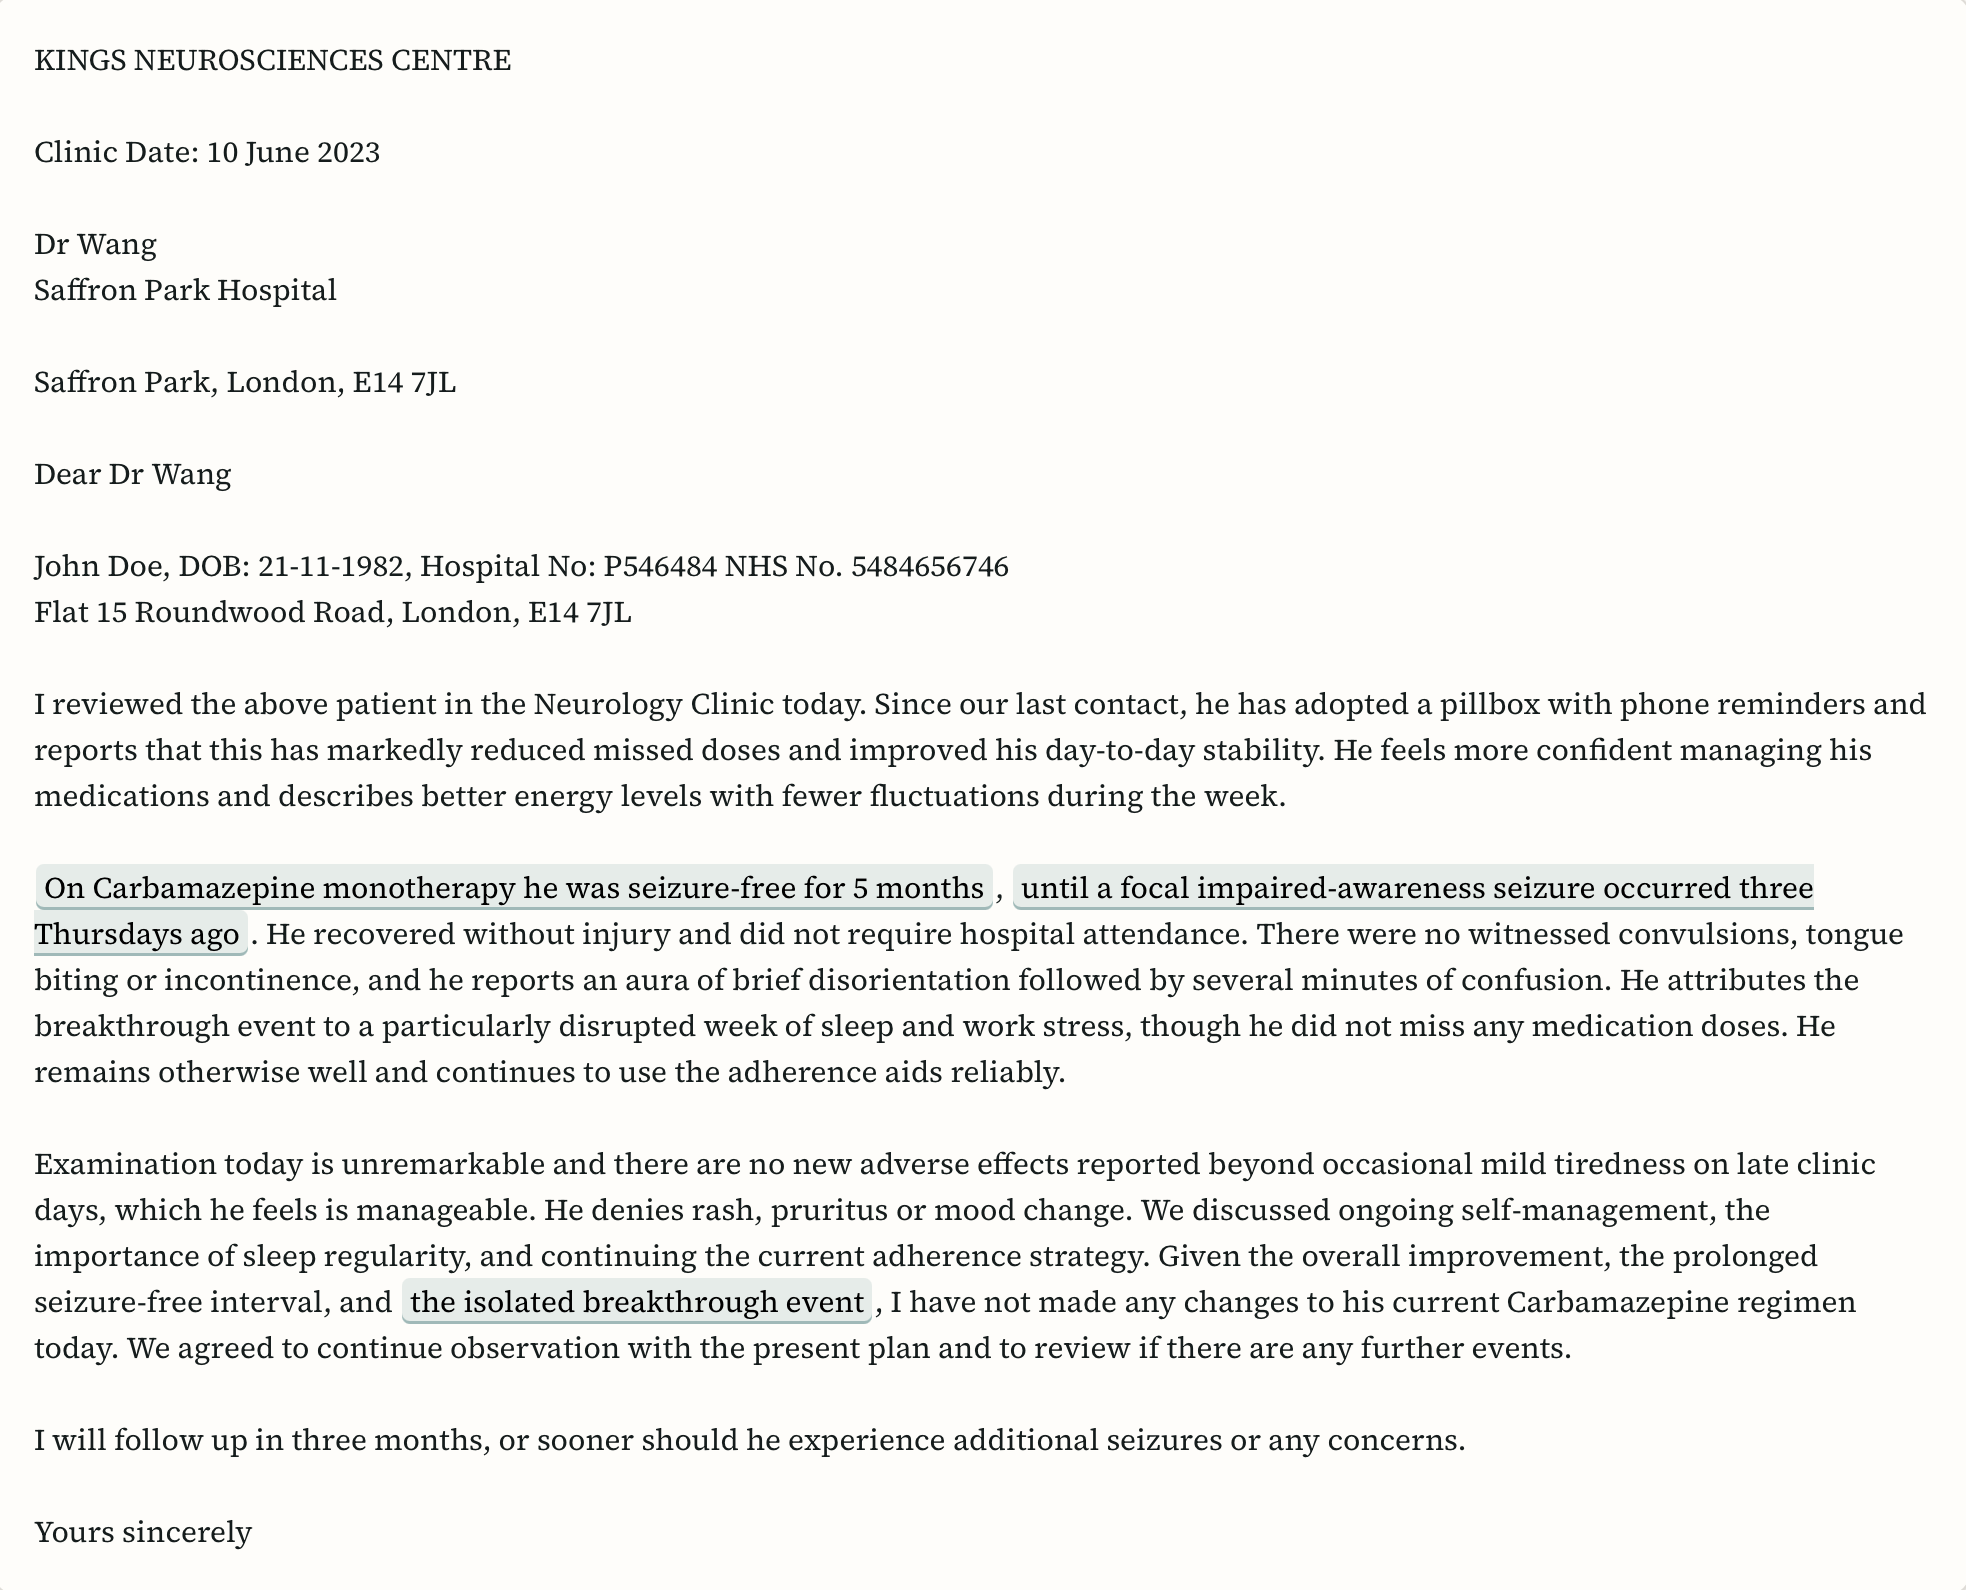
\includegraphics[width=\linewidth]{fig2.png}
        \caption{Example clinical letter from King's College Hospital with relevant seizure frequency events highlighted.}
        \label{fig:second}
    \end{subfigure}

    \caption{Example clinical letters from Swansea Bay (a) and King's College Hospital (b). Highlighted sections of the letter illustrate the areas where the pipeline identified relevant clinical facts for the task.}
    \label{fig:combined}
\end{figure*}

\subsection{Architecture}

\section{Results}
\subsection{Development Environment}
\subsection{Methods}
\subsection{Models}
\subsection{Structured Evidence}
\subsection{Ablations}
\subsection{Error Analysis}

\section{Discussion}

\section{Conclusion}

\begin{tabularx}{\linewidth}{|Y|Y|Y|Y|}
\hline
\textbf{Entity} &
\textbf{Claim it supports} &
\textbf{Evidence shown} &
\textbf{Reviewer risk} \\
\hline

Table 1: Dataset Summary &
Method is robust and generalisable &
Dataset size, labels, splits, class balance &
How valuable is synthetic data? \\
\hline

Table 2: Main Results &
Method improves over baseline in 3 key ways &
F1, evidence, schema validity, uncertainty &
What do schema and evidence validity mean? \\
\hline

Figure 1: Architecture &
Method is modular, transparent, reproducible, and clinically logical &
Pipeline stages, representative example &
Architecture may seem unnecessarily convoluted \\
\hline

Table 3: Ablation &
Deterministic and LLM components are complementary &
LLM-only, rules-only, LLM + schema validation, LLM + evidence verifier,
LLM + concept normalisation, LLM + temporal resolver, full hybrid &
Unclear separation between rules and LLM; unclear rules \\
\hline

Figure 2: Error Analysis &
Deterministic and LLM components have distinct error profiles that you can calibrate for &
Hallucinations, low recall, schema validity, evidence coverage,
normalisation errors, temporal contradiction, abstention rate &
Difficulty identifying the most meaningful errors \\
\hline
\end{tabularx}

\section*{References}

Please number citations consecutively within brackets \cite{b1}. The 
sentence punctuation follows the bracket \cite{b2}. 

\begin{thebibliography}{00}
\bibitem{b1} B. Fonferko-Shadrach \emph{et al.}, ``Using natural language processing to extract structured epilepsy data from unstructured clinic letters: development and validation of the ExECT (extraction of epilepsy clinical text) system,'' \emph{BMJ Open}, vol.~9, no.~4, 2019, Art.~no.~e023232.
\bibitem{b2} B. Fonferko-Shadrach \emph{et al.}, ``Annotation of epilepsy clinic letters for natural language processing,'' \emph{J. Biomed. Semantics}, vol.~15, no.~17, 2024.
\bibitem{b3} K. Xie \emph{et al.}, ``Extracting seizure frequency from epilepsy clinic notes: a machine reading approach to natural language processing,'' \emph{J. Amer. Med. Informat. Assoc.}, vol.~29, no.~5, pp.~873--881, 2022.
\bibitem{b4} B. Holgate, J. Davies, S. Fang, J.~S. Winston, J.~T. Teo, and M.~P. Richardson, ``Fine-tuning LLMs to extract epilepsy seizure frequency data from health records,'' in \emph{Proc. 24th Workshop on Biomedical Language Processing (BioNLP)}, 2025, pp.~44--55.
\bibitem{b5} Y. Gan \emph{et al.}, ``Reproducible synthetic clinical letters for seizure frequency information extraction,'' arXiv:2603.11407, 2026.
\bibitem{b6} S. Fu \emph{et al.}, ``Clinical concept extraction: A methodology review,'' \emph{J. Biomed. Informat.}, vol.~109, 2020, Art.~no.~103526.
\bibitem{b7} R. Grishman and B. Sundheim, ``Message Understanding Conference-6: A brief history,'' in \emph{Proc. 16th Int. Conf. Computational Linguistics (COLING)}, 1996, pp.~466--471.
\bibitem{b8} Y. Wang \emph{et al.}, ``Clinical information extraction applications: A literature review,'' \emph{J. Biomed. Informat.}, vol.~77, pp.~34--49, 2018.
\bibitem{b9} K. Xie, B. Litt, D. Roth, and C.~A. Ellis, ``Quantifying clinical outcome measures in patients with epilepsy using the electronic health record,'' in \emph{Proc. BioNLP Workshop}, 2022, pp.~369--375.
\bibitem{b10} M. Agrawal, S. Hegselmann, H. Lang, Y. Kim, and D. Sontag, ``Large language models are few-shot clinical information extractors,'' in \emph{Proc. Conf. Empirical Methods in Natural Language Processing (EMNLP)}, 2022, pp.~1998--2022.
\bibitem{b11} L. Chiticariu, Y. Li, and F. Reiss, ``Rule-based information extraction is dead! Long live rule-based information extraction systems!,'' in \emph{Proc. Conf. Empirical Methods in Natural Language Processing (EMNLP)}, 2013, pp.~827--832.
\bibitem{b12} B.~M. Decker \emph{et al.}, ``Development of a natural language processing algorithm to extract seizure types and frequencies from the electronic health record,'' \emph{Seizure}, vol.~101, pp.~48--51, 2022.
\end{thebibliography}

\vspace{12pt}
\color{red}
IEEE conference templates contain guidance text for composing and formatting conference papers. Please ensure that all template text is removed from your conference paper prior to submission to the conference. Failure to remove the template text from your paper may result in your paper not being published.

\end{document}
